
\section{Getexample Outline}

The main aim of the \emph{getexample} is to provide easy access to the examples for the users. For this reason, the getexample tool is expected to be 
have the following design specifications:

\begin{figure}[!ht]
\begin{center}
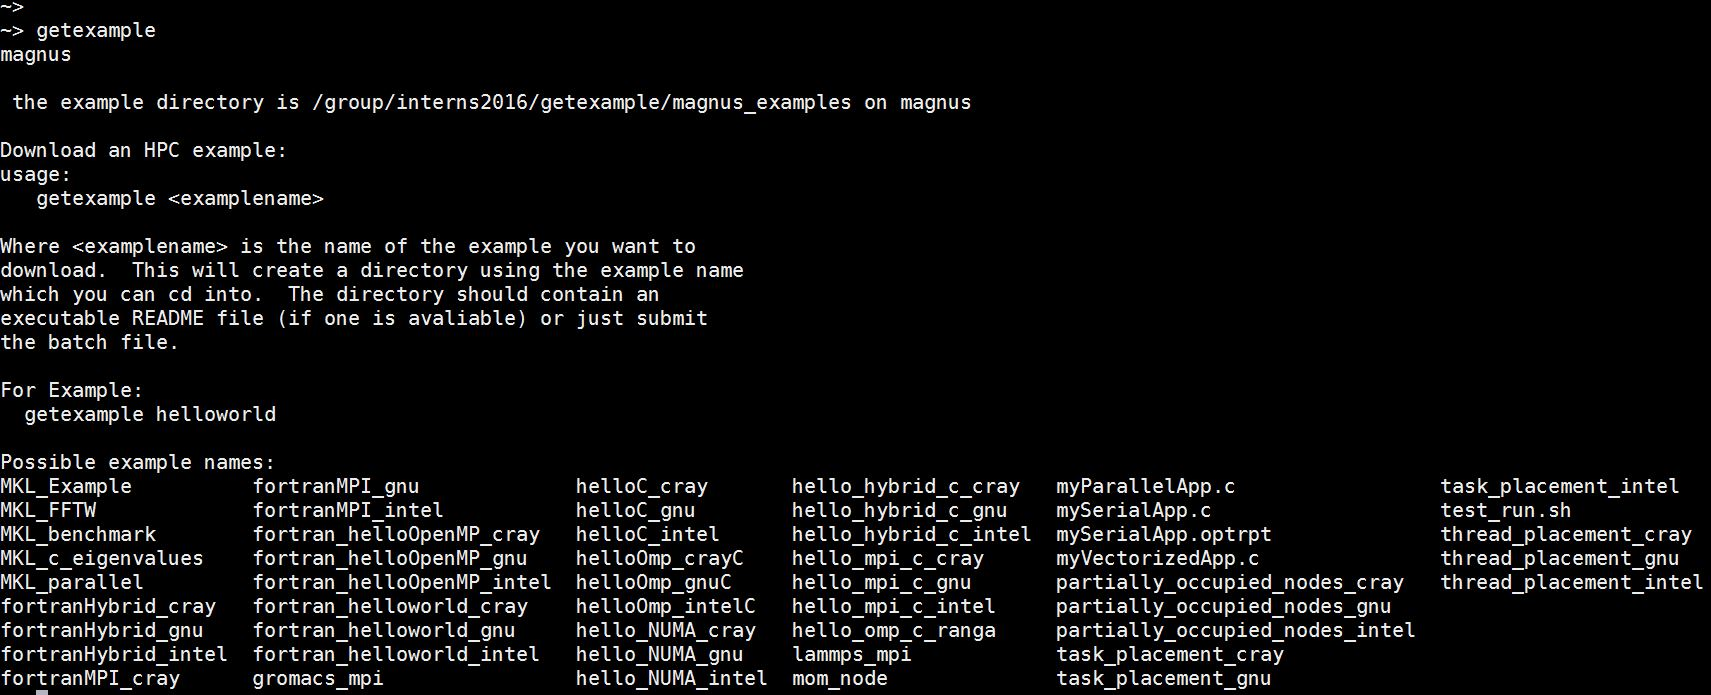
\includegraphics[scale=0.6]{getexample}
\caption{The Listing of Examples when typed "getexample" on Magnus}
%\label{dataset1}
\end{center}
\end{figure}

\begin{figure}[!ht]
\begin{center}
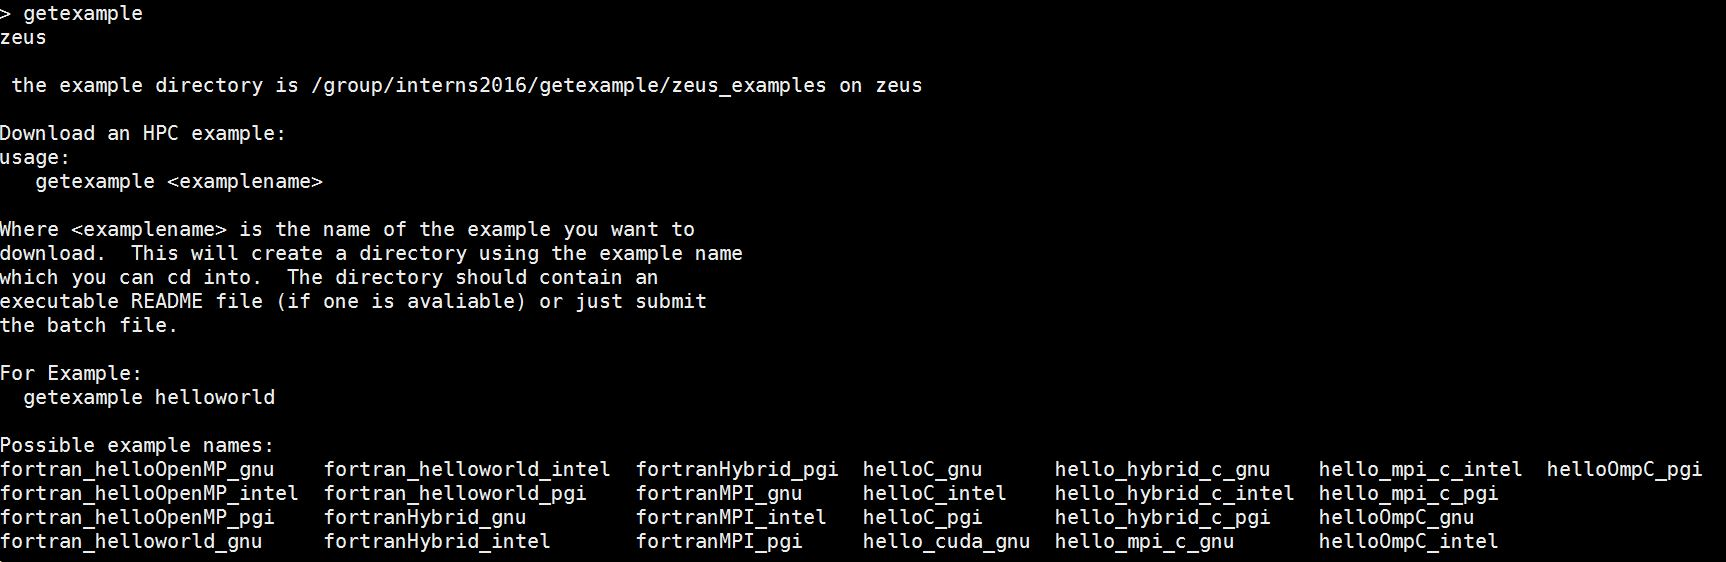
\includegraphics[scale=0.61]{getexamplezeus}
\caption{The Listing of Examples when typed "getexample" on Zeus}
%\label{dataset1}
\end{center}
\end{figure}

\begin{figure}[!ht]
\begin{center}
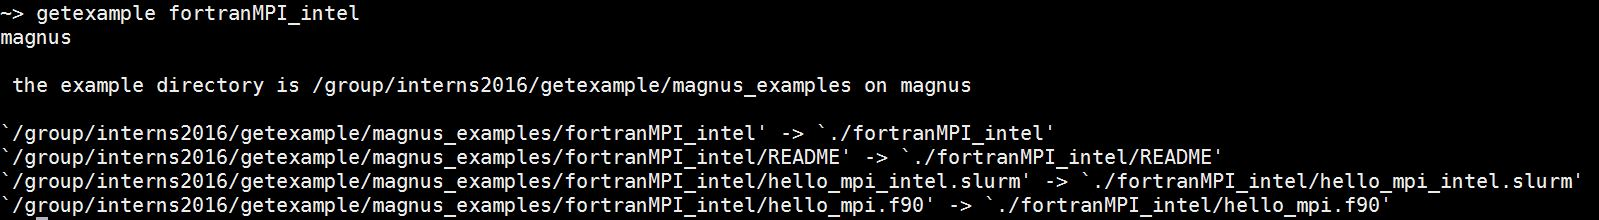
\includegraphics[scale=0.63]{getexamplehybrid}
\caption{Feedback given to the user while downloading the example}
%\label{dataset1}
\end{center}
\end{figure}

\begin{figure}[!ht]
\begin{center}
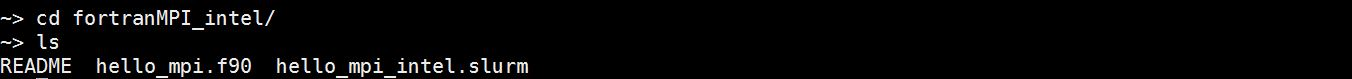
\includegraphics[scale=0.70]{files}
\caption{The List of files in the fortranHybrid\_intel directory}
%\label{dataset1}
\end{center}
\end{figure}

\clearpage

\begin{itemize}
\item It should be easy to use for everyone including beginners. The user should be able to download the examples and run them with one command.
\item It should provide practical examples which can be modified or updated by the users for their own work. Therefore, it encourages the users to learn
how to use the resources given to them effectively.
\item The examples should be clear and completely detailed with steps to help the users understand and apply it.
\end{itemize}

The getexample tool is designed in a way such that when \emph{getexample} command is typed from any directory on the resources of Pawsey Centre, it 
lists all the examples within the getexample library as shown in Fig. 1 on the previous page. As the getexample displays many examples which aim to 
perform various tasks for each individual resource at Pawsey, it ensures that when the user logins from a specific supercomputer such as Magnus, it 
only lists the examples provided for Magnus rather than showing all of the examples within the library. To obtain a copy of any example, the user simply 
types \emph{getexample} followed by the name of the example as shown below:

\begin{tcolorbox}
\begin{Verbatim}[fontsize=\scriptsize]
getexample <name of the example>
\end{Verbatim}
\end{tcolorbox}

This creates a new directory with same name as the example requested in wherever the getexample tool is accessed from and it downloads all the files of
the example to the new directory created and gives a feedback to the user about what the command is doing as shown in Fig. 2. The new directory then can 
be accessed by the user simply typing:

\begin{tcolorbox}
\begin{Verbatim}[fontsize=\scriptsize]
cd <name of the example>
\end{Verbatim}
\end{tcolorbox}

As mentioned earlier, each example consists of 3 files which are the README and SLURM scripts, and the source code as shown in Fig. 3 on the previous
page.


